\documentclass{article}
\usepackage[utf8]{inputenc}
\usepackage{graphicx}
\usepackage[version=4]{mhchem}

% ── Cross-reference to ESI ────────────────────────────────────────────────────
% Requires esi.aux to exist (compile esi.tex before the second pass of main.tex).
% All ESI labels are accessible with the prefix "S-", e.g. \ref{S-fig:multi_corr_exp}.
\usepackage{xr}
\externaldocument[S-]{esi}

% additional packages
\usepackage{color}
\usepackage{siunitx}
\usepackage{amssymb}
\usepackage{booktabs}
\usepackage{threeparttable}

% Units

\DeclareSIUnit{\angstrom}{\text{\AA}}

% References and abbreviations
\newcommand*{\eg}{\emph{e.g. }}
\newcommand*{\etal}{\emph{et al.}}
\newcommand*{\ie}{\emph{i.e. }}
\newcommand*{\reffig}[1]{Fig.~\ref{#1}}
\newcommand*{\refsec}[1]{Section~\ref{#1}}
\newcommand*{\refeq}[1]{Eq.~\ref{#1}}
\newcommand*{\reftab}[1]{Table.~\ref{#1}}

% Symbols for physics
\newcommand*{\dcp}{d_{\mathrm{cp}}}
\newcommand*{\phieff}{\phi_{\mathrm{eff}}}
\newcommand*{\dsg}{d_{\mathrm{sg}}}
\newcommand*{\dion}{d_{\mathrm{ion}}}
\newcommand*{\deff}{d_{\mathrm{eff}}}
\newcommand*{\nsg}{N_{\mathrm{sg}}}
\newcommand*{\npp}{N_{\mathrm{PP}}}
\newcommand*{\nnp}{N_{\mathrm{NP}}}
\newcommand*{\qpp}{q_{\mathrm{PP}}}
\newcommand*{\qnp}{q_{\mathrm{NP}}}
\newcommand*{\nup}{N_{\mathrm{UP}}}
\newcommand*{\qup}{q_{\mathrm{UP}}}
\newcommand*{\qp}{q_{\mathrm{p}}}
\newcommand*{\np}{N^{\mathrm{p}}}
\newcommand*{\npsg}{N^{\mathrm{p}}_{\mathrm{sg}}}
\newcommand*{\pnpsg}{P^{\np}_{\npsg}}
\newcommand*{\pzz}{P^{0}_{0}}
\newcommand*{\poe}{P^{1}_{8}}
\newcommand*{\pte}{P^{2}_{8}}
\newcommand*{\pn}{P^\mathrm{n}}
\newcommand*{\lbox}{L_\mathrm{box}}
\newcommand*{\vp}{\phi_\mathrm{p}}
\newcommand*{\nmi}{N_{\mathrm{mi}}}
\newcommand*{\ncl}{N_{\ce{Cl-}}}
\newcommand*{\nna}{N_{\ce{Na+}}}
\newcommand*{\acl}{a_{\ce{Cl-}}}
\newcommand*{\ana}{a_{\ce{Na+}}}
\newcommand*{\anacl}{a_{\ce{NaCl}}}
\newcommand*{\ccl}{c_{\ce{Cl-}}}
\newcommand*{\cna}{c_{\ce{Na+}}}
\newcommand*{\gpm}{\gamma_{\pm}}
\newcommand*{\dpex}{\Delta p_\mathrm{excess}}
\newcommand*{\dptot}{\Delta p^\mathrm{osm}_\mathrm{total}}
\newcommand*{\dpid}{\Delta p_\mathrm{ideal}}
\newcommand*{\pex}{p_\mathrm{excess}}
\newcommand*{\ptot}{p^\mathrm{osm}_\mathrm{total}}
\newcommand*{\pid}{p_\mathrm{ideal}}
\newcommand*{\dl}{\kappa^{-1}}
\newcommand*{\bulk}{\mathrm{bulk}}
\newcommand*{\neutral}{\mathrm{neutral}}
\newcommand*{\cppm}{\mathrm{CPPM}}
\newcommand*{\csalt}{c_\mathrm{salt}}

\title{Ion Asymmetry and Electrostatic Screening in Dense Solutions of Patchy Macroions}

\author{Sebastian Pineda, Mikael Lund}
\date{}

\begin{document}

\maketitle

\begin{abstract}
We study concentrated suspensions of Charged Patchy Particle Model (CPPM) macroions — coarse-grained protein analogues with systematically varied surface charge distributions — using grand-canonical Monte Carlo simulations with explicit \ce{NaCl} salt at a volume fraction of $\vp = 0.30$ and salt activity $\anacl = \qty{100}{mM}$.
By comparing explicit-ion and implicit-ion (Yukawa-screened) simulations across four CPPM variants differing in the spatial arrangement of surface charges, we quantify how charge anisotropy shapes osmotic pressure, ion partitioning, and structural correlations.
We find that increasing charge anisotropy — from isotropic $\pzz$ to dipolar $\poe$ to quadrupolar $\pte$ — promotes orientational ordering that lowers the osmotic pressure and redistributes counterions asymmetrically around the macroion surface.
Fitting the implicit-ion $g(r)$ to the explicit-ion reference reveals that the optimal Debye screening length substantially exceeds the theoretical Debye--Hückel value for the isotropic variant, for which no single screening length adequately reproduces the explicit-ion structure.
These results clarify when and why the implicit-ion approximation breaks down in crowded protein solutions, and identify packing-driven structure as the primary obstacle to the Yukawa description of uniformly charged macroions.
\end{abstract}

\section{\label{sec:intro} Introduction}

The interior of a living cell is far from a dilute aqueous solution.
The cytoplasm of \textit{E.\ coli} contains roughly \qty{350}{\mg\per\mL} of macromolecules, placing it firmly in the crowded regime where excluded-volume and electrostatic interactions between proteins are strong and persistent~\cite{wennerstrom_colloidal_2020}.
Wennerström \etal argued that the colloidal stability of a cell is not primarily governed by specific interactions but by a collective electrostatic repulsion between macromolecules: the overwhelming majority of cytosolic proteins carry a net negative surface charge density of roughly $-1e$ per \qty{11}{\nm\squared}, sufficient to generate a long-range repulsion that counteracts aggregation~\cite{wennerstrom_colloidal_2020}.
What makes this argument distinctive is the ionic environment in which it operates.
The intracellular concentration of free, small monovalent ions is estimated to be only $\sim\!\qty{20}{mM}$ — much lower than the \qty{150}{mM} \ce{NaCl} of a typical buffer — because most anions are sequestered in macromolecular structures.
The resulting Debye length ($\dl \approx \qty{22}{\angstrom}$) is nearly three times longer than in buffer ($\dl \approx \qty{8}{\angstrom}$), substantially extending the range of electrostatic repulsion and supporting colloidal stability through a Donnan-like redistribution of mobile ions.

Real proteins, however, are not uniformly charged spheres.
High-resolution structural studies reveal that surface charge groups are distributed asymmetrically, giving every protein a characteristic multipole signature~\cite{bozic2017a}.
This charge anisotropy is not merely a structural curiosity: it couples to rotational degrees of freedom, and therefore to orientational pair correlations, osmotic pressure, and the effective interactions that govern phase behaviour.
The importance of surface charge patches has been underscored by studies on antibodies, where regions of positive charge flanked by a negatively charged surface promote non-specific self-association and drive liquid--liquid phase separation~\cite{ausserwoger2023}.
Patchy charge distributions thus go beyond modifying pair potentials: they create orientationally selective interactions that cannot be captured by an effective spherically symmetric potential~\cite{yigit2015a,yigit2017a}.

The Charged Patchy Particle Model (CPPM), originally introduced by Yigit \etal~\cite{yigit2015a}, provides a controlled minimal model to isolate the effect of charge distribution on colloidal properties.
By rearranging the same number of charges on an otherwise identical sphere, one obtains a family of model proteins spanning isotropic ($\pzz$), dipolar ($\poe$), and quadrupolar ($\pte$) charge distributions, all at the same net charge.
This controlled parameter variation enables a direct comparison of thermodynamic and structural observables as a function of charge patchiness, free of the confounding variations in size, hydrophobicity, and total charge that complicate comparisons between real proteins.
The multipole expansion of the electrostatic interaction energy — formalized through the dipole moment vector~\cite{bozic2017a} and traceless quadrupole tensor, and discussed in the context of charge regulation by Podgornik and coworkers~\cite{podgornik2018a} — provides the natural framework for quantifying the hierarchy of charge asymmetry across CPPM variants.
Charge patchiness also underpins the patchy-particle picture of colloidal self-assembly~\cite{bianchi2025}, where directional, valence-limited interactions from charge heterogeneity drive network formation and cluster equilibria in ways qualitatively different from isotropic potentials.

A central practical question for simulating crowded protein solutions is whether explicit mobile ions are necessary, or whether a screened Coulomb (Yukawa/Debye--Hückel) potential between macroions, parameterized by a single effective Debye screening length $\dl$, captures the relevant physics.
Implicit-ion simulations are orders of magnitude cheaper, and work well for uniformly charged colloids at low to moderate concentrations and salt.
However, at the high macroion densities relevant to crowded cellular environments, and for proteins with significant charge heterogeneity, the mean-field approximation underlying the Yukawa model may fail.
Recent experimental and simulation evidence suggests that implicit-ion models cannot reproduce the structure and self-association behaviour of antibodies with marked charge patchiness, while explicit-ion simulations recover the correct thermodynamics~\cite{ausserwoger2023}.
For CPPMs, Yigit \etal~\cite{yigit2015a} showed that ion distributions around a single patchy macroion are strongly anisotropic, with counterions clustering near like-charged surface regions; this structured ion atmosphere is qualitatively different from the isotropic Debye cloud assumed in the implicit model.
The effective screening length that would best reproduce the explicit-ion structural properties is therefore expected to deviate from the Debye--Hückel prediction based on the nominal salt concentration, and that deviation should depend on the degree of charge patchiness.

In this article we address this question systematically by comparing explicit- and implicit-ion grand-canonical MC simulations of concentrated CPPM solutions at the four levels of charge anisotropy.
We characterize the osmotic pressure and its decomposition into ideal and excess contributions, orientational pair correlations, spatial distribution functions of salt ions around the macroion surface, and the accuracy of the multipole expansion relative to the exact pairwise electrostatic energy.
By fitting the implicit-ion radial distribution function $g(r)$ to the explicit-ion reference, we identify the best-matching screening length $\dl_*$ for each variant and compare it to both the theoretical Debye--Hückel prediction at the nominal ionic strength and to the effective screening length that accounts for Donnan partitioning of counterions.
The results provide a clear picture of when and how charge anisotropy determines the validity of the implicit-ion approximation in dense macroion suspensions.

\section{Methods}
\label{sec:methods}

\subsection{Molecular simulations}

We studied structural properties and orientational correlations of concentrated macro-ion solutions using Metropolis Monte Carlo (MC) simulations implemented in Faunus~\cite{stenqvist2013}.
The macro-ion solution was modeled with the Charged Patchy Particle Model (CPPM)~\cite{yigit2015a}, representing the dense intracellular environment~\cite{wennerstrom_colloidal_2020}.
Two electrolyte treatments were employed: (a)~explicit-ion simulations with grand-canonical \ce{NaCl} and (b)~implicit-ion simulations with a Yukawa-screened Coulomb potential parameterized by the Debye screening length $\dl$.
The best $\dl$ reproducing the explicit-ion structure was identified by minimizing the peak absolute deviation $|\Delta g|_\text{max}$ of the CPPM--CPPM radial distribution function $g(r)$.
All simulation input files, output trajectories, and analysis scripts are available from the Zenodo repository: (?).

\subsubsection{Charged Patchy Particle Model (CPPM)}

The CPPM consists of a center uncharged particle (CP) with diameter $\dcp = \qty{40}{\angstrom}$ decorated with $\nsg = 66$ surface groups with diameter $\dsg = \qty{4}{\angstrom}$.
Surface groups are of three types: negative (NP, $\qnp = -1e$), positive (PP, $\qpp = +1e$), and uncharged (UP, $\qup = 0$).
We studied four variants: three with $\nnp=37$ and $\npp=29$ giving net charge $\qp = -8e$ ($\pzz$, $\poe$, $\pte$), and one fully neutral variant ($\pn$, $\nup=66$).
The charge distributions range from isotropic ($\pzz$) to dipolar ($\poe$, one positive patch of 8 groups) and quadrupolar ($\pte$, two patches of 8 groups each); for full construction details see Ref.~\cite{yigit2015a}.

The dipole moment vector is defined as
\begin{equation}
    \vec{\mu} = \sum_i q_i \vec{r}_i,
    \label{eq:dipole}
\end{equation}
where $q_i$ is the charge and $\vec{r}_i$ the position of surface group $i$ relative to the center of the CPPM.
The traceless quadrupole tensor is
\begin{equation}
    \mathbf{Q} = \frac{1}{2}\sum_i q_i
    \left( 3\,\vec{r}_i \otimes \vec{r}_i - |\vec{r}_i|^2 \mathbf{I} \right),
    \label{eq:quadrupole}
\end{equation}
with Frobenius norm
\begin{equation}
    \Theta = \|\mathbf{Q}\|_F = \sqrt{\sum_{j,k} Q_{jk}^2}.
    \label{eq:frobenius}
\end{equation}

\reffig{fig:cppms} shows the coarse-grained representation of the charged CPPM variants with their surface charge density projected onto a plane using the Mollweide projection.
The net charge, the magnitude of the dipole moment $\mu$ and the Frobenius norm of the traceless quadrupole tensor $\Theta$ are listed in the top panel for each variant.
Each point charge is smeared with a von Mises--Fisher kernel ($\lambda = 20$, angular half-width ${\approx}15^\circ$).
Although $\pzz$ is designed to have a uniform charge distribution, the discrete placement of a finite number of charges results in a small but non-zero dipole and quadrupole moment, as shown in panel (a).
These residual moments are not expected to drive orientational correlations.
The markers in each panel indicate the position of the poles of the dipole moment vector as well as the two antipodal poles of the prolate axis of the traceless quadrupole tensor (largest positive eigenvalue), and the oblate axis (most negative eigenvalue).

\begin{figure}
    \centering
    \includegraphics[width=1\textwidth]{figs/cppm-table_MW.png}
    \caption{(Top) Coarse-grained representation of the charged CPPM variants: $\pzz$, $\poe$ and $\pte$ along with the net charge, the magnitude of the dipole moment $\mu$ and the Frobenius norm of the traceless quadrupole tensor $\Theta$.
    Color coding: gray = center particle, red = positive surface group, blue = negative surface group.
    (Bottom) Surface charge density mapped onto the unit sphere via the Mollweide equal-area projection where the charges are smeared with a spherical smoothing kernel.
    All projections share a common color scale anchored to the model with the widest density range.
    White squares ($\square$) indicate the two poles of the dipole moment.
    White triangles ($\vartriangle$/$\triangledown$) indicate the two antipodal poles of the prolate axis of quadrupole tensor, and black triangles ($\blacktriangle$/$\blacktriangledown$) the oblate axis.
    Marker size scales qualitatively with the magnitude of the corresponding moment.}
    \label{fig:cppms}
\end{figure}

\subsubsection{Simulation system and interaction potentials}

All systems consisted of $\nmi = 30$ rigid macro-ions in a cubic simulation box ($\lbox = \qty{149.64}{\angstrom}$, $\vp = 0.30$) with a dielectric continuum solvent ($\varepsilon_r = 78.36$, $T = \qty{298.15}{\kelvin}$).
A simulation snapshot is shown in ESI \reffig{S-fig:snapshot}.
In the explicit-ion runs, monovalent \ce{Na+}/\ce{Cl-} ions ($\dion = \qty{4}{\angstrom}$, $\pm e$) were maintained at salt activity $\qty{0.1}{M}$ by GCMC insertion/deletion of ion pairs; charged variants accommodated $\langle\nna\rangle = 300$ and $\langle\ncl\rangle = 60$ on average, the neutral variant $\langle\nna\rangle = \langle\ncl\rangle = 123$.
In the implicit-ion runs the Yukawa screened potential
\begin{equation}
    u_{ij}(r) = k_{\rm B}T \, \frac{q_i \, q_j \, \ell_{\rm B}}{r} \, e^{-\kappa r},
    \label{eq:yukawa}
\end{equation}
replaced explicit ions, with Bjerrum length $\ell_{\rm B} = \qty{7.153}{\angstrom}$ at \qty{298.15}{\kelvin}.
Simulations were performed over the $\dl$ ranges listed in \reftab{tab:kappa}; short-range repulsions used the WCA potential with Lorentz--Berthelot combining rules.
Full simulation protocol details are given in ESI Sec.~\ref{S-esi:sec:simdetails}.

\begin{table}[htbp]
    \centering
    \caption{Range of simulated Debye screening lengths $\dl$ for each CPPM variant. All simulations used $n_\text{rep} = 3$ independent replicas. The theoretical value $\dl_\mathrm{th} = \qty{9.61}{\angstrom}$ corresponding to the equilibrated free ionic strength was simulated additionally for all variants.}
    \label{tab:kappa}
    \begin{tabular}{lccc}
        \toprule
        Variant & $\dl_\text{min}$ (\AA) &
                  $\dl_\text{max}$ (\AA) &
                  $n_{\dl}$ \\
        \midrule
        $\pzz$  & 10.0 & 37.9 & 20 \\
        $\poe$  & 10.5 & 14.3 &  6 \\
        $\pte$  & 12.5 & 16.7 &  6 \\
        $\pn$   & 14.3 & 40.0 &  3 \\
        \bottomrule
    \end{tabular}
\end{table}

\subsubsection{Analysis}

CPPM--CPPM $g(r)$ functions were computed from centers of mass, and the optimal implicit-ion screening length was identified by minimizing $|\Delta g|_\text{max}$ against the explicit-ion reference (restricted to $r \geq \qty{40.0}{\angstrom}$).
The analytical Percus--Yevick hard-sphere $g(r)$ was used as a structural reference, with effective diameter $\deff$ fitted to the neutral CPPM $g(r)$.
Orientational and multipole-energy correlations were decomposed into ion--ion, ion--dipole, dipole--dipole, and ion--quadrupole contributions up to order $r^{-3}$:
\begin{align}
    u_{ii} &= k_{\rm B}T\,\ell_{\rm B}\,\frac{q_i\,q_j}{r},
    \label{eq:u_ii}\\
    u_{id} &= k_{\rm B}T\,\frac{\ell_{\rm B}}{r^2}
               \bigl[q_i\,(\vec{\mu}_j\cdot\hat{r}_{ij})
                    +q_j\,(\vec{\mu}_i\cdot\hat{r}_{ij})\bigr],
    \label{eq:u_id}\\
    u_{dd} &= k_{\rm B}T\,\frac{\ell_{\rm B}}{r^3}
               \bigl[\vec{\mu}_i\cdot\vec{\mu}_j
                    -3(\vec{\mu}_i\cdot\hat{r}_{ij})
                      (\vec{\mu}_j\cdot\hat{r}_{ij})\bigr],
    \label{eq:u_dd}\\
    u_{iq} &= k_{\rm B}T\,\frac{3\,\ell_{\rm B}}{2r^3}
            \bigl[q_i\,(\hat{r}_{ij}\cdot\mathbf{Q}_j\cdot\hat{r}_{ij})
            +q_j\,(\hat{r}_{ij}\cdot\mathbf{Q}_i\cdot\hat{r}_{ij})\bigr].
    \label{eq:u_iq}
\end{align}
Three-dimensional spatial distribution functions, osmotic pressure, and mean activity coefficients were also computed; full methodological details are provided in ESI Sec.~\ref{S-esi:sec:simdetails}.

\section{Results and Discussion}

\subsection{Explicit-ion simulations}

\subsubsection{Thermodynamic analysis \label{sec:ther_ana}}

\reffig{fig:deltap} shows the osmotic pressure increment $\dptot$ relative to the bulk \ce{NaCl} reference for all four CPPM variants.
All systems yield a net positive $\dptot$, confirming that the dense CPPM suspensions exert a net repulsive osmotic response.
Strikingly, $\dptot$ decreases monotonically with increasing charge anisotropy: the isotropic variant $\pzz$ generates the highest increment, the dipolar $\poe$ and quadrupolar $\pte$ are progressively lower, and $\pte$ produces an increment indistinguishable from the neutral $\pn$ system, despite the latter carrying no surface charge whatsoever.
This decrease arises from reductions in both the ideal ($\dpid$) and excess ($\dpex$) contributions, as shown by the bar decomposition in \reffig{fig:deltap}.

The ideal pressure increments reveal a clear signature of charge-driven ion partitioning.
For the neutral system, both sodium and chloride contribute equally negative ideal increments ($\dpid^{\ce{Na+}} = \dpid^{\ce{Cl-}} < 0$), reflecting a symmetric depletion of both species from the macro-ion solution caused purely by steric exclusion.
For the three charged variants, sodium contributes positively ($\dpid^{\ce{Na+}} > 0$) while chloride contributes negatively ($\dpid^{\ce{Cl-}} < 0$), reflecting the Donnan partitioning: the negatively charged macro-ion surface draws excess counterions (Na$^+$) into the system while partially excluding co-ions (Cl$^-$).
Importantly, the degree of this asymmetry differs among the three charged variants even though all carry the same net charge $\qp = -8e$, implying that the spatial arrangement of charges — and the resulting dipole and quadrupole moments — influences counterion partitioning beyond what is captured by the net charge alone.
The structural origin of these differences is investigated in Subsection~\ref{sec:struc_ana}.

The mean activity coefficients (\reftab{tab:gamma}) tell a complementary story.
The bulk electrolyte gives $\gpm^\bulk = 0.85$, consistent with the standard Debye--Hückel prediction for 0.1~M NaCl ($\gpm \approx 0.78$) and reflecting net attractive correlations between Na$^+$--Cl$^-$ pairs.
The neutral system gives $\gpm^\neutral = 1.57$, a large positive deviation indicating that the macro-ion excluded volume and short-range repulsions strongly suppress ion--ion correlations.
The three charged variants all have $\gpm \approx 1.0$, suggesting near-ideal behavior of the small ions.
This apparent ideality is, however, a macroscopic average over a microscopically heterogeneous system: as discussed in Subsection~\ref{sec:struc_ana}, the charged macro-ion surface strongly localizes counterions while depleting co-ions, and the two effects approximately cancel in the activity coefficient, masking the underlying microscopic non-uniformity.

The excess osmotic pressure increments $\dpex$ reflect the total effect of macro-ion--macro-ion and macro-ion--ion interactions.
The isotropic $\pzz$ produces the largest $\dpex$, exceeding even the neutral $\pn$ system, which suggests that the uniform negative charge distribution adds a net repulsive contribution on top of the hard-core packing present in all systems.
The dipolar $\poe$ and quadrupolar $\pte$ show lower $\dpex$ relative to the neutral, indicating that the favorable charge--patch interactions — ion-dipole and dipole-dipole terms — partially compensate the repulsive packing, reducing the net excess pressure.
These trends are consistent with the structural and orientational analysis in Subsection~\ref{sec:struc_ana}, and their microscopic origin is further examined through the pairwise energy decomposition presented in \reffig{S-fig:multi_ene_exp} in the ESI.

\begin{figure}
    \centering
    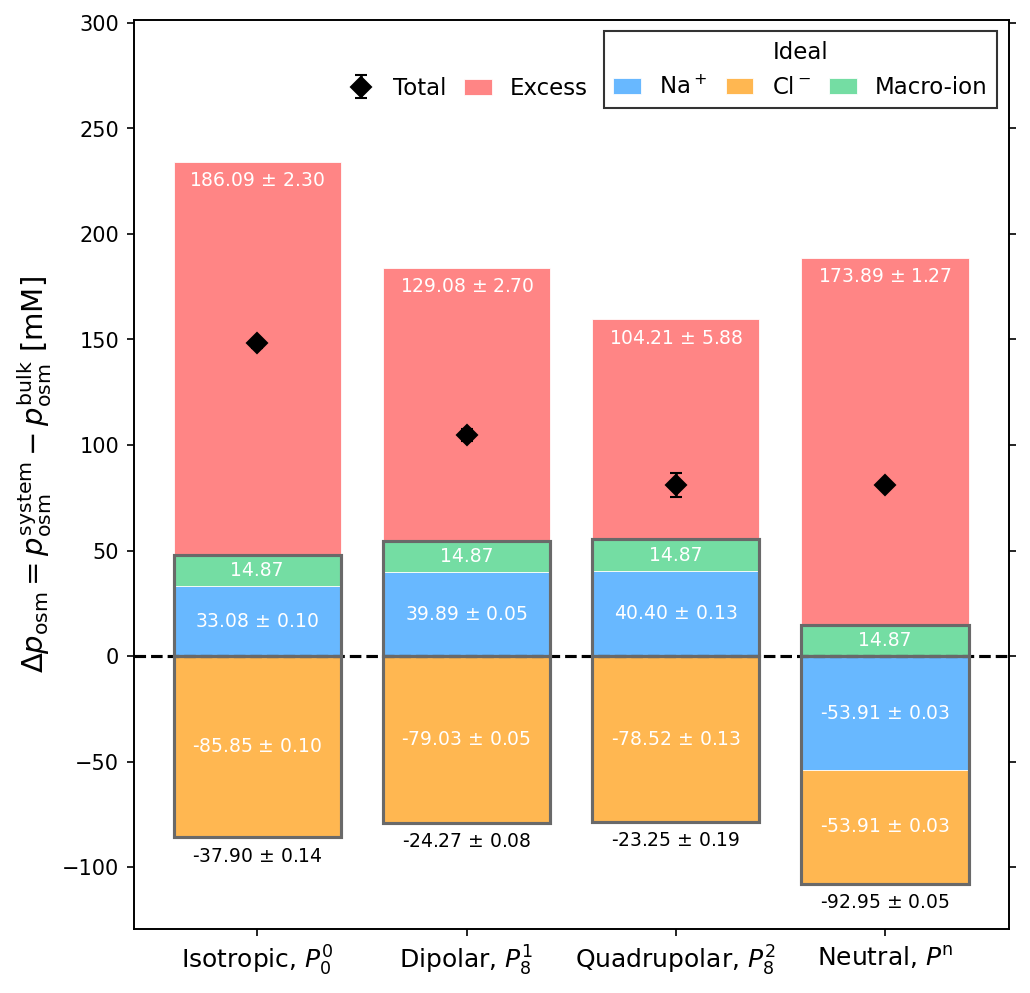
\includegraphics[width=0.7\textwidth]{figs/pressure_stacked.png}
    \caption{Decomposition of the osmotic pressure increment for explicit-ion CPPM solutions relative to a \ce{NaCl} bulk reference of activity $\anacl = \qty{100}{mM}$.
    Diamond markers show the total increment $\Delta\ptot$ with propagated uncertainty.
    Each bar is partitioned into the ideal contributions of \ce{Na+}, \ce{Cl-}, and the macro-ion (boxed group), and the excess pressure; segment values (mean~$\pm$~SD) are printed in white, and the total ideal sum ($\Delta\pid$) is printed below the outlined block.}
    \label{fig:deltap}
\end{figure}

\begin{table}[htbp]
    \centering
    \begin{tabular}{cccccc}
        \toprule
        System & Bulk & Isotropic, $\pzz$ & Dipolar, $\poe$ & Quadrupolar, $\pte$ & Neutral, $\pn$  \\
        \midrule
        $\gpm$ & 0.85 & 1.10              & 1.02            & 1.01                & 1.57            \\
        \bottomrule
    \end{tabular}
    \caption{Mean activity coefficient $\gpm$ of small ions in aqueous CPPM solutions at volume fraction of $\vp = 0.30$ and \ce{NaCl} activity of $\anacl = \qty{100}{mM}$.}
    \label{tab:gamma}
\end{table}

\subsubsection{Structural analysis \label{sec:struc_ana}}

\reffig{fig:gofr_exp} compares the center-of-mass CPPM--CPPM radial distribution functions $g(r)$ for the four variants at contact.
The most striking observation is the strong dependence of both peak height and peak shape on charge anisotropy.
The quadrupolar $\pte$ reaches the highest first-shell peak ($g_\text{max} = 4.65$ at $r \approx \qty{43.1}{\angstrom}$), followed by the dipolar $\poe$ ($g_\text{max} = 3.62$), the neutral $\pn$ ($g_\text{max} = 2.80$), and the isotropic $\pzz$ ($g_\text{max} = 2.30$).
Remarkably, the isotropic variant produces a lower first-shell peak than the fully uncharged neutral system, indicating that the uniform negative surface charge of $\pzz$ adds a repulsive contribution that suppresses contact-pair formation relative to the purely steric neutral system.

The shape of the first-shell peak provides additional insight.
The dipolar $\poe$ and quadrupolar $\pte$ systems exhibit narrow, nearly Gaussian peaks, which are the hallmark of orientationally driven pairing: a preferred relative orientation creates a well-defined approach geometry, and the orientational order vanishes quickly beyond the first shell, causing $g(r)$ to return smoothly to unity.
In contrast, the isotropic $\pzz$ and neutral $\pn$ systems show a broader peak with an approximately linear decay, consistent with the hard-sphere-like structure expected at high volume fractions.
This packing-driven behavior is confirmed by the Percus--Yevick fit to the neutral $g(r)$, which yields an effective hard-sphere diameter $\deff = \qty{42.9}{\angstrom}$ (effective volume fraction $\phieff = 0.37$) and reproduces the key structural features qualitatively.

The orientational pair correlations (\reffig{S-fig:multi_corr_exp} in the ESI) support this interpretation quantitatively.
At first-shell contact ($r \approx \qty{44}{\angstrom}$), the isotropic $\pzz$ shows essentially no orientational order in any metric ($|\text{correlation}| < 0.02$ for all four measures), confirming that the packing-dominated structure of this system carries no orientational memory.
The dipolar $\poe$ exhibits a significant positive dipole--dipole correlation ($\langle\hat{\mu}_i\cdot\hat{\mu}_j\rangle \approx 0.17$) and positive longitudinal projection ($\langle(\hat{\mu}_i\cdot\hat{r}_{ij})(\hat{\mu}_j\cdot\hat{r}_{ij})\rangle \approx 0.19$), indicating a tendency for head-to-tail dipole alignment — the electrostatically preferred configuration — and a mild quadrupole--quadrupole anti-alignment ($-0.085$).
The quadrupolar $\pte$, by contrast, has negligible dipole--dipole correlation ($< 0.01$) but a substantially negative quadrupole--quadrupole correlation ($\langle\hat{\mathbf{Q}}_i{:}\hat{\mathbf{Q}}_j\rangle \approx -0.19$), revealing a dominant anti-aligned quadrupolar ordering at contact that decays over $r \approx \qty{55}{\angstrom}$.
All orientational correlations decay to noise ($< 0.02$) by $r \gtrsim \qty{55}{\angstrom}$, confirming that the orientational order is a contact-shell phenomenon.

The spatial distribution functions shown in \reffig{fig:3d_sdfs} reveal the microscopic ion distribution around each CPPM variant.
For the charged variants, sodium counterions cover a considerably larger surface area than chloride co-ions, consistent with the net negative macro-ion charge.
In the isotropic $\pzz$ system, sodium ions are distributed approximately uniformly over the surface while chloride ions appear as a sparse, broadly distributed cloud — a picture consistent with a structureless but net-attracting counterion atmosphere.
The dipolar $\poe$ and quadrupolar $\pte$ systems show a qualitatively different pattern: chloride ions concentrate in dense, well-localized clouds directly above the positively charged patches, while sodium ions cover the remainder of the surface.
This selective accumulation of co-ions above positive patches confirms that the spatial arrangement of surface charges, not just the net charge, determines how the small-ion atmosphere is organized.

For the dipolar $\poe$ system, the spatial distribution of neighboring CPPM surface groups (\reffig{fig:3d_sdfs},b) reveals two additional features: a localized negative-bead isosurface sitting nearly on top of the positive patch — overlapping with the chloride cloud — and a positive-bead isosurface displaced to the equatorial region.
This geometry is consistent with two coexisting pairing motifs: a direct CPPM--CPPM interaction in which the negative patch of one macro-ion faces the positive patch of its neighbor, and a salt-mediated pathway in which a transient chloride cloud above the positive patch bridges to the positive-patch region of a second macro-ion.
The orientational correlations favor the direct mode, but the salt-mediated mechanism may provide an additional pathway that reduces the effective repulsion.
A similar analysis for the quadrupolar $\pte$ system (\reffig{fig:3d_sdfs},c) shows four positive-bead and two negative-bead neighbor isosurfaces arranged symmetrically about the two patch axes, consistent with the dominant anti-aligned quadrupolar ordering identified in the correlation analysis.
The absence of chloride bridging clouds deep between the positive patches in $\pte$ (in contrast to $\poe$) suggests that the two closely spaced patches in the quadrupolar system create a more tightly coupled direct CPPM--CPPM interaction with less salt mediation.
The neutral system shows uniform, structureless ion distributions for both species, confirming the absence of any charge-driven selectivity.

Taken together, these results establish that charge anisotropy shapes colloidal structure not only through modifications to the effective pair potential, but also through the coupling between the macro-ion charge pattern and the local small-ion organization.
The favorable orientational arrangements in the anisotropic variants reduce both the ideal (via Donnan partitioning shifts) and the excess (via favorable short-range pairing) contributions to the osmotic pressure, producing the monotonic decrease in $\dptot$ with increasing anisotropy observed in \reffig{fig:deltap}.
Conversely, the isotropic variant, despite its high net charge, develops no orientational ordering, and the structure is dominated by hard-core packing at the high volume fraction $\vp = 0.30$, leading to the largest excess pressure increment among all charged variants.

\begin{figure}
    \centering
    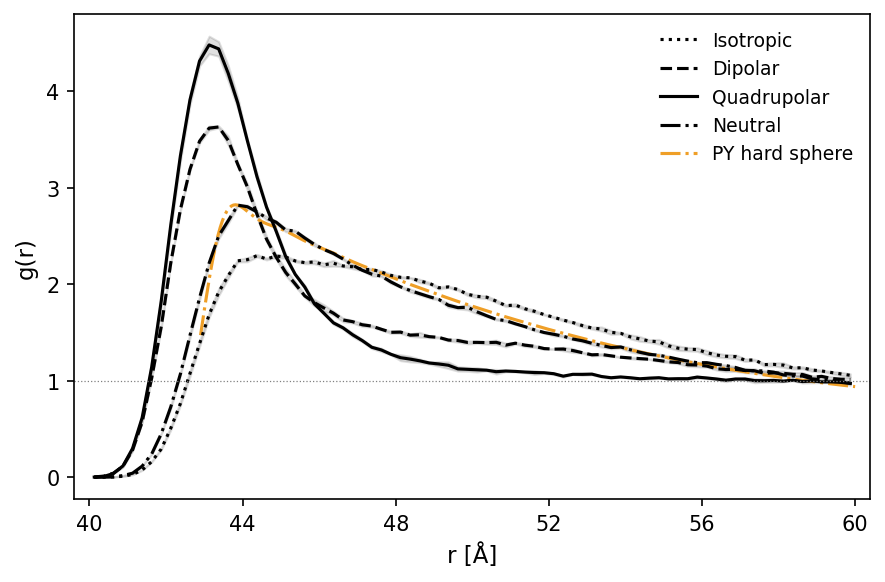
\includegraphics[width=1\textwidth]{figs/rdf_explicit_overlay_black.png}
    \caption{Center-of-mass radial distribution functions $g(r)$ of the CPPM variants: $\pzz$ (dotted), $\poe$ (dashed), $\pte$ (solid) and $\pn$ (dash-dotted) obtained from explicit-ion simulations at volume fraction of $\vp = 0.30$ and \ce{NaCl} activity of $\anacl = \qty{100}{mM}$.
    The orange dash-dotted line shows the Percus--Yevick hard-sphere theory fitted to the $\pn$ system (effective diameter $\deff = \qty{42.9}{\angstrom}$, $\phieff = 0.37$).}
    \label{fig:gofr_exp}
\end{figure}

\begin{figure}
    \centering
    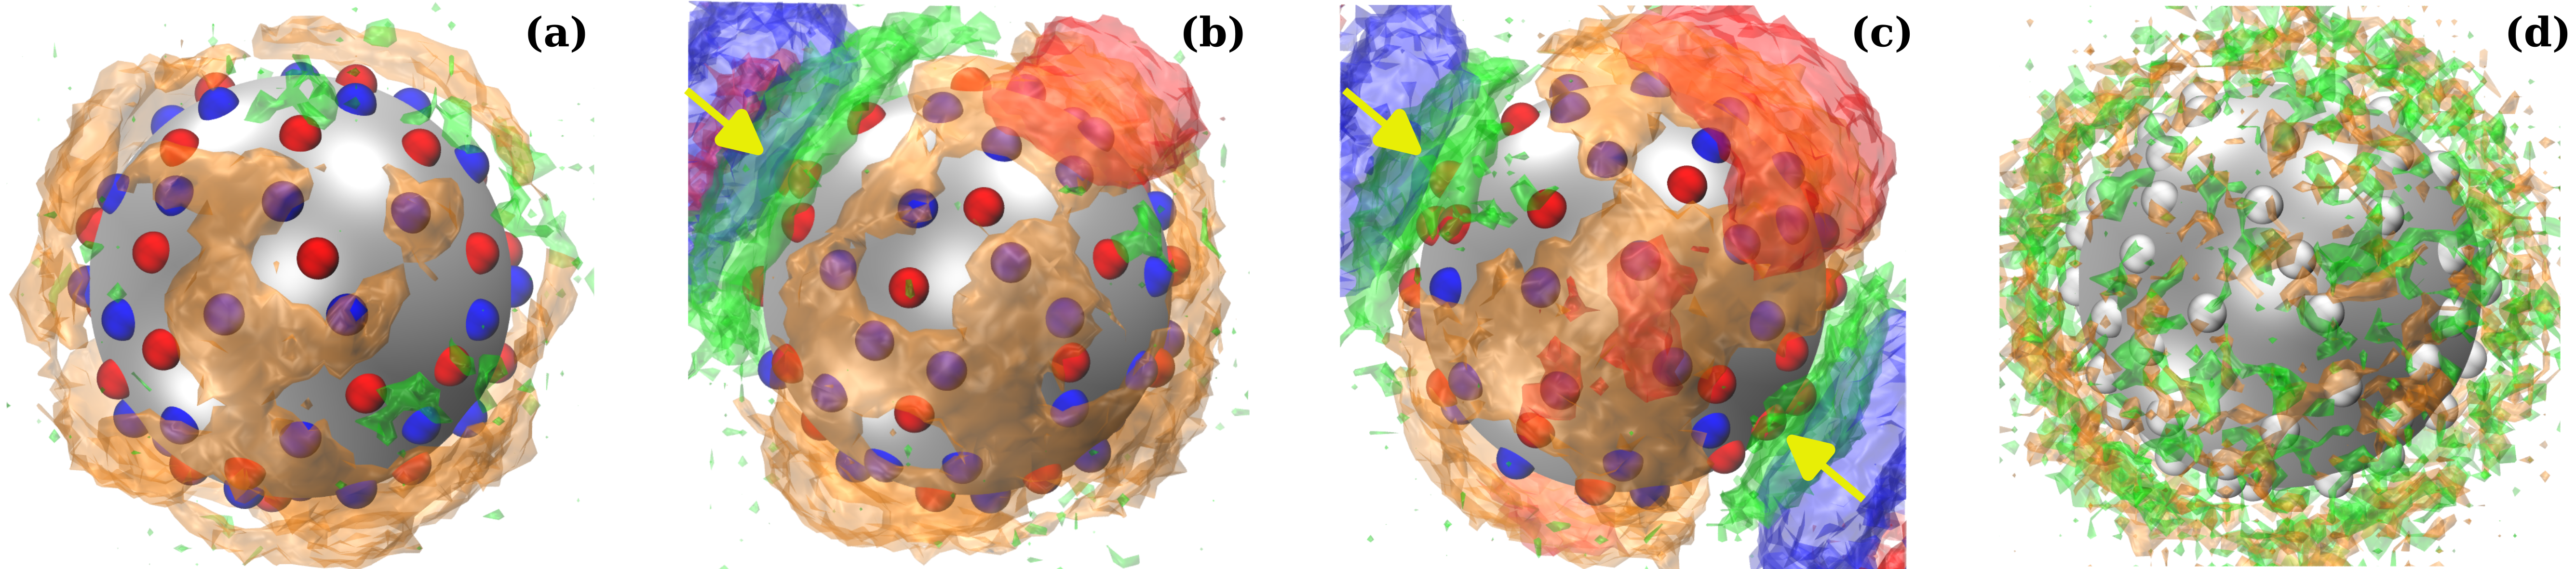
\includegraphics[width=1\textwidth]{figs/sdfs.png}
    \caption{Spatial distribution of salt ions and surface groups around the CPPM variants: (a) $\pzz$, (b) $\poe$, (c) $\pte$ and (d) $\pn$.
    Isosurfaces correspond to normalized local densities of 1.3 (surface groups) and 2.3 (ions) for the charged variants.
    For the neutral variant, the lower local density of 1.75 (ions) was used to render the more weakly structured distribution.
    Yellow arrows indicate the position of the center of the positively charged patches.
    Color coding: gray = center particle, red = positive surface groups, blue = negative surface groups, orange = sodium ions, green = chloride ions.
    }
    \label{fig:3d_sdfs}
\end{figure}

\subsection{Comparison of explicit- and implicit-ion simulations \label{sec:impl}}

\subsubsection{Screening-length scan \label{sec:dl_scan}}

Having characterized the explicit-ion behavior in detail, we now ask whether an implicit-ion simulation with a suitably chosen Debye screening length $\dl$ can reproduce the explicit-ion structural properties.
\reffig{S-fig:gofr_com} (ESI) shows the CPPM--CPPM $g(r)$ from implicit-ion simulations over the full $\dl$ scan, overlaid with the explicit-ion reference.
The qualitative trends are informative: for the dipolar $\poe$ and quadrupolar $\pte$ variants, there exists a range of $\dl$ values for which the implicit-ion $g(r)$ is close to the explicit-ion reference, including the correct peak height and decay shape.
For the isotropic $\pzz$, however, the implicit-ion peak height is systematically above the explicit-ion reference at every value of $\dl$ across the entire scan ($\dl = 10.0$--$37.9$~\AA).
As $\dl$ decreases (stronger screening), the implicit-ion peak grows higher, so the best agreement is at the weakest screening tested.
At the strongest screening ($\dl_\mathrm{th} = \qty{9.61}{\angstrom}$ corresponding to $I = \qty{0.1}{M}$) the implicit simulation is considerably more structured than the explicit reference.

This behavior has a clear physical interpretation.
In the explicit simulation, the negative macro-ion surface attracts sodium counterions that form a dense, partially neutralizing cloud, effectively reducing the net charge seen by a neighboring macro-ion.
The implicit-ion model, using the full net charge $\qp = -8e$ but exponential screening, cannot replicate this charge renormalization: at any fixed $\dl$, it either over-screens (at short $\dl$) or under-screens (at long $\dl$) the effective potential, and the resulting $g(r)$ is too structured in both cases.
For the isotropic system, this fundamental inadequacy is compounded by the fact that structure at $\vp = 0.30$ is largely packing-driven: the hard-sphere-like nature of the $\pzz$ $g(r)$ means that even moderate changes in the electrostatic term cannot shift the contact peak by the amount required to match the explicit-ion reference.

The neutral $\pn$ $g(r)$ is, by construction, insensitive to $\dl$ since it carries no surface charge, and we confirmed that all three simulated screening lengths yield essentially the same $g(r)$ peak ($2.80 \pm 0.02$), consistent with a structure governed entirely by excluded volume.

\subsubsection{Optimal screening length and comparison with theory \label{sec:best_kappa}}

\reffig{fig:bestk} compares the implicit-ion $g(r)$ at the best-fit screening length $\dl_*$ (minimizing the peak absolute deviation $|\Delta g|_\text{max}$) and at the theoretical value $\dl_\mathrm{th} = \qty{9.61}{\angstrom}$ against the explicit-ion reference for the three charged variants.

For the dipolar $\poe$ variant, the best-fit screening length is $\dl_* = \qty{12.5}{\angstrom}$ (corresponding to $\kappa_* = \qty{0.080}{\per\angstrom}$).
At this value, the implicit-ion $g(r)$ reproduces the explicit-ion peak height and general shape remarkably well, with residuals remaining below $\Delta g \approx 0.1$ at all separations.
The theoretical $\dl_\mathrm{th} = \qty{9.61}{\angstrom}$, derived from the nominal salt activity of \qty{100}{mM}, produces a noticeably over-structured $g(r)$, with a peak approximately 0.3 units too high.

For the quadrupolar $\pte$ variant, $\dl_* = \qty{16.7}{\angstrom}$ ($\kappa_* = \qty{0.060}{\per\angstrom}$).
The agreement at $\dl_*$ is very good, with the implicit-ion $g(r)$ reproducing the peak height $g_\text{max} = 4.65$ and the broad first-shell feature of $\pte$.
At $\dl_\mathrm{th}$, the quadrupolar system is again over-structured, with a peak deviation comparable to that seen for the dipolar system.

For the isotropic $\pzz$ variant, the best-fit at $\dl_* = \qty{37.9}{\angstrom}$ (the weakest screening tested) still overestimates the explicit-ion peak by approximately $\Delta g \approx 0.16$, and the residual profile does not exhibit a clear minimum within the simulated range.
No single Debye screening length can reconcile the implicit-ion structure with the explicit-ion reference for this variant.

The optimal screening lengths $\dl_* = 12.5$ and \qty{16.7}{\angstrom} for the dipolar and quadrupolar systems, respectively, are both substantially longer than the nominal $\dl_\mathrm{th} = \qty{9.61}{\angstrom}$.
This systematic shift is expected from the Donnan equilibrium: in a solution of $\nmi = 30$ macro-ions with $\qp = -8e$, charge neutrality requires 240 excess sodium ions that do not participate in the free electrolyte.
With approximately $\nna = 300$ sodium and $\ncl = 60$ chloride ions in the simulation box (volume $V = L^3 = \qty{3.35e6}{\angstrom\cubed}$), the free ionic strength contributed by paired \ce{NaCl} is only $\csalt \approx \qty{30}{mM}$, giving an effective Debye length of $\dl_\mathrm{eff} = 3.04/\sqrt{0.030} \approx \qty{17.5}{\angstrom}$.
This estimate is in close agreement with the best-fit $\dl_* = \qty{16.7}{\angstrom}$ for the quadrupolar variant, and in reasonable agreement with $\dl_* = \qty{12.5}{\angstrom}$ for the dipolar.
The shorter optimal $\dl_*$ for the dipolar system relative to the quadrupolar may reflect the role of orientational correlations: the head-to-tail dipole alignment concentrates positive and negative patches in close proximity, partially screening the effective repulsion at contact and requiring a somewhat stronger implicit screening to match the explicit-ion peak height.

The failure of the implicit-ion model for the isotropic variant merits further discussion.
In that system, both the charge distribution and the resulting ion atmosphere are spherically symmetric; as the simulation confirms, no orientational order develops.
Structure at the high volume fraction $\vp = 0.30$ is therefore almost entirely packing-driven, as evidenced by the near-perfect PY hard-sphere description of the neutral $g(r)$ and by the visual similarity between the $\pzz$ and $\pn$ peak profiles.
In such a packing-dominated regime, the Yukawa screening length primarily controls the amplitude of the first peak, but the explicit-ion simulation produces a peak lower than any implicit simulation because the diffuse counterion cloud effectively reduces the net macro-ion charge below $-8e$.
The implicit-ion model, fixing the charge at its nominal value, is structurally stiffer at any $\dl$, and no choice of $\dl$ within a physically reasonable range compensates for this renormalization.
This is consistent with the coupling-parameter argument: the electrostatic coupling $\Gamma = \ell_\mathrm{B} \, q_p^2 / \dl \approx 47$ for the net charge and $\dl = \dl_\mathrm{th}$ places the system in a regime where mean-field Debye--Hückel theory is expected to overestimate repulsion, precisely the trend we observe.

The orientational correlation functions at $\dl_*$ (\reffig{S-fig:mp_corr_best} in the ESI) further confirm that the implicit-ion simulations at the best-fit screening length recover the correct orientational order for the dipolar and quadrupolar systems: the dipole--dipole correlation and head-to-tail projection for $\poe$, and the quadrupole--quadrupole anti-alignment for $\pte$, match the explicit-ion reference closely at $\dl_*$.
At $\dl_\mathrm{th}$, orientational correlations are generally stronger than in the explicit reference, consistent with the over-structured $g(r)$.
For the isotropic $\pzz$, the implicit-ion orientational correlations remain negligible at all $\dl$, in agreement with the explicit reference.

\begin{figure}
    \centering
    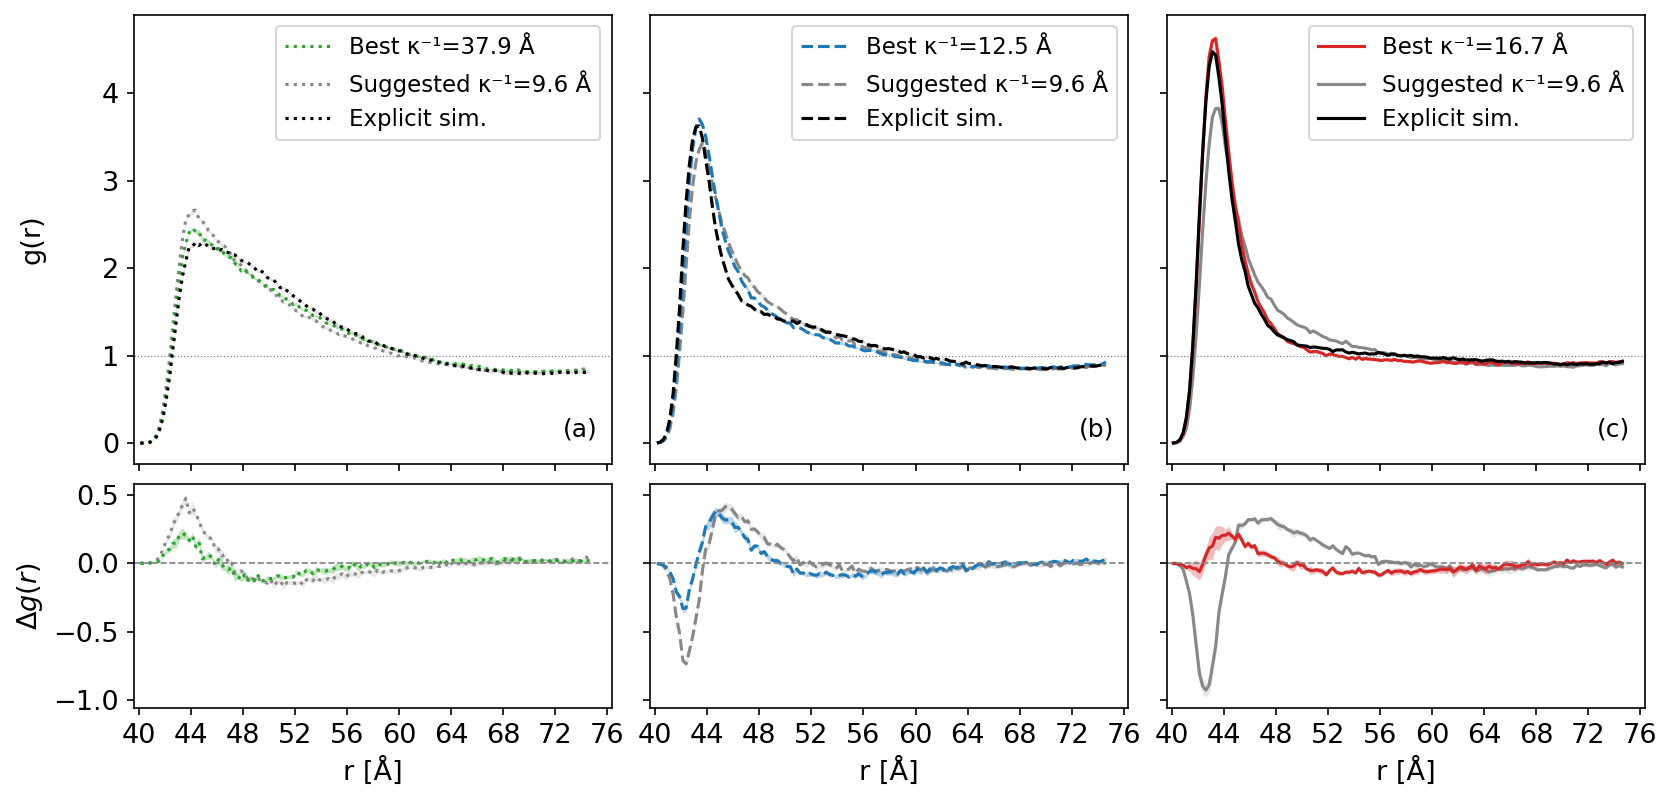
\includegraphics[width=1\textwidth]{figs/best_kappa_comparison_1x3.png}
    \caption{Radial distribution functions $g(r)$ at the best-fit Debye screening length $\dl_*$ for the three charged CPPM variants: (a)~$\pzz$ ($\dl_* = \qty{37.9}{\angstrom}$, dotted), (b)~$\poe$ ($\dl_* = \qty{12.5}{\angstrom}$, dashed), and (c)~$\pte$ ($\dl_* = \qty{16.7}{\angstrom}$, solid).
    Upper sub-panel: implicit-ion $g(r)$ at $\dl_*$ (colored lines); implicit-ion $g(r)$ at the screening length $\dl_\mathrm{th} = \qty{9.61}{\angstrom}$ predicted from the explicit-ion ionic strength (gray); and the explicit-ion reference (black lines).
    Shaded bands indicate the mean $\pm$ SEM across replicas.
    Lower sub-panel: residuals $\Delta g(r) = g_\mathrm{imp}(r) - g_\mathrm{exp}(r)$ with propagated uncertainty; the horizontal gray dashed line marks zero.}
    \label{fig:bestk}
\end{figure}

\section{Conclusion}

We have shown that charge anisotropy in dense macro-ion suspensions controls both thermodynamic and structural properties in ways that go beyond what the net charge alone would predict.
At a volume fraction of $\vp = 0.30$, the osmotic pressure increment decreases monotonically as the charge distribution becomes more anisotropic, from the isotropic variant to the quadrupolar one, because favorable orientational correlations reduce the excess pressure contribution.
The spatial distribution of small ions around the macro-ion surface mirrors this behavior: charge patches generate strongly localized counterion and co-ion clouds, and the coupling between patch geometry and ionic organization drives distinct pairing motifs — direct charge-patch contacts and salt-mediated bridging — that collectively lower the repulsive response of the system.

The comparison between explicit- and implicit-ion simulations reveals a clear hierarchy of model validity.
For the dipolar and quadrupolar CPPM variants, a single effective Debye screening length reproduces the explicit-ion $g(r)$ well, but the optimal value ($\dl_* \approx 12.5$--$\qty{16.7}{\angstrom}$) substantially exceeds the nominal Debye--Hückel value at \qty{100}{mM} ($\dl_\mathrm{th} = \qty{9.61}{\angstrom}$).
The longer effective screening length is explained quantitatively by the Donnan equilibrium: the net negative macro-ions draw a large excess of sodium counterions into the solution, reducing the free electrolyte concentration from \qty{100}{mM} to approximately \qty{30}{mM} and raising the effective Debye length to $\sim\!\qty{17.5}{\angstrom}$.
For the quadrupolar system this Donnan-corrected estimate is essentially exact; for the dipolar system the optimal $\dl_*$ is somewhat shorter, which we attribute to the head-to-tail dipole alignment at contact that partially screens the effective inter-patch repulsion.
For the isotropic variant, by contrast, no implicit-ion simulation within a physically reasonable range of screening lengths reproduces the explicit-ion $g(r)$: packing effects dominate at $\vp = 0.30$ and the charge renormalization from the counterion cloud cannot be captured by a fixed-charge Yukawa potential at any single $\dl$.

These results have practical implications for the simulation of crowded protein solutions.
When charge anisotropy is significant, as in dipolar and quadrupolar proteins, the implicit-ion model with a Donnan-corrected screening length provides a computationally efficient and structurally accurate approximation.
For nearly isotropic proteins at high volume fractions, however, the accuracy of the Yukawa model should be treated with caution: the dominant packing effects and strong charge renormalization make the choice of $\dl$ relatively inconsequential, and a dedicated explicit-ion simulation is needed to capture the correct structure.
This distinction is relevant to the cellular context motivated in the Introduction, where the long intracellular Debye length and the high macromolecular crowding place the system precisely in the regime where the implicit-ion approximation is most likely to fail for isotropic macroions while remaining useful for anisotropic ones.


\bibliographystyle{unsrt}
\bibliography{pmc}

\end{document}
